%!TEX root = ../template.tex
%%%%%%%%%%%%%%%%%%%%%%%%%%%%%%%%%%%%%%%%%%%%%%%%%%%%%%%%%%%%%%%%%%%%
%% chapter3.tex
%% NOVA thesis document file
%%
%% Chapter with a short laext tutorial and examples
%%%%%%%%%%%%%%%%%%%%%%%%%%%%%%%%%%%%%%%%%%%%%%%%%%%%%%%%%%%%%%%%%%%%

%%-------------------------------------------------------------------
%%	3 - Proposed Work
%%-------------------------------------------------------------------
\chapter{Proposed Work}
\label{cha:proposed_work}

This chapter firstly presents the technologies that will serve as the basis for the development of the work proposed in the following section. Then is given an overview of the solution and finally, there is a presentation of a detailed action plan.

%%-------------------------------------------------------------------
%%	2.2. - Existing Technologies
%%-------------------------------------------------------------------
\section{Existing Technologies} % (fold)
\label{sec:existing_technologies}
This section briefly lists the main technologies the work will be built upon.

\begin{description}
	\item [BTRFS] is a modern file system built from scratch, initially designed by Oracle Corporation, based on the copy-on-write principle. This file system aims at implementing advanced features while also focusing on fault tolerance, repair and easy administration. But its most interesting feature is its ability to create snapshots of directories and files. Btrfs uses B + trees as the main structure for storing the data. Everything in this file system, from inodes, to data, directories, along with others, is an object in the B + tree.
	%
	\item [Memcached~\cite{github_memcached}] is an open source, high-performance, distributed memory object caching system. It acts as an in-memory key-value store for small arbitrary data (such as strings or objects) from results of database calls, API calls, or page rendering. This tool is constituted by four major components: 1) Client software that has a list of available memcached servers;  2) A client-based hashing algorithm, which chooses a server based on the key;  3) Server software, which stores values with their keys into an internal hash table; 4) Least Recently Used cache which determines when to throw out old data.
\end{description}


% section existing_technologies (end)

%%-------------------------------------------------------------------
%%	3. - Proposed Solution
%%-------------------------------------------------------------------
\section{Proposed Solution} % (fold)
\label{sec:proposed_solution}

This work focuses on the problematic of storing virtual machines in a context of virtual desktop infrastructure, in this sequence the general idea is to introduce a replication and caching system with basis on a local file system. Moreover, this solution should integrate correctly with the existing platform using the part of the infrastructure which is already functional.
There are three fundamental steps to the realisation of this project towards accomplishing all the goals.\footnotemark

\footnotetext{At the time of writing, these are the goals that make sense to us. Still, the architecture of this solution is dependent on consultation with Reditus S.A, a discussion that will only occur after the deadline of this document.}

First, there is a need for some preliminary evaluation. 
As already mentioned, this project has been underway for quite some time. In this sense, now that it is the moment to change from a single-node paradigm to a multi-node one, even having in mind a multi-site distribution, the demand for a thorough study is in order. This examination is intended to understand in detail the current operation of the storage infrastructure, and what happens when users use the platform asking for files and put some pressure on the system. This phase is of great importance since its results will be decisive for the following design phases and general shape of the solution.


Addressing the second requirement originates the need to tackle the challenge of introducing a caching system to storage servers. In this design, a client of the storage system will first check if what is being requested is within the cache system and only in case of a cache miss will the request be routed to the layer below. The difficulty here is that this system must put up with reasonably large files resulting from the consolidation of snapshots in a distributed environment.
There are some solutions currently in the market such as Memcached, where support is more focused on making small files available, but there is the possibility of tweaking the system for the sake of getting it to work with bigger files.

There are some relevant issues when talking about a single-node solution, such as low fault tolerance, a general scaling difficulty, and limited availability. Here the approach focuses on the idea of replicating a BTRFS-based file system and at the same time ensuring the properties just mentioned.
Two methodologies can be followed to complete this objective. One is to use an existing middleware and integrate it with the different components of the infrastructure. The second is to build from scratch a solution that fulfils this requirement. At the moment it is not yet decided which of the approaches to take, but this will be one of the main objectives of the design phase of the solution.

We plan to evaluate our work in a setting that includes servers running on a platform provided by Reditus S.A and featuring the complete iCBD solution. Thus being able to conduct a series of benchmarks in a near real-world setting. Such test can be grouped into three parameter categories to study, the required bandwidth, latency presented and the number of input/output operations per second (IOPS). Comparing these categories according to various types of operations (sequential reading, random reading, sequential writing, random writing) in order to simulate multiple types of workload that may occur in a deployment of this platform. 
To this end, we expect to be able to use an open-source tool called  Flexible I/O Tester (fio)~\cite{github_fio} that mitigates the need of writing tailored test cases and allows the use of job files containing the operating environment that needs to be tested.
In addition, it is necessary to evaluate the behaviour of the solution in a virtualized environment with several nodes, including fault tolerance correction and general availability.

% section proposed_solution (end)



%%-------------------------------------------------------------------
%%	3. - Work Plan
%%-------------------------------------------------------------------
\section{Work Plan} % (fold)
\label{sec:work_plan}

In this section the work plan for the elaboration of the dissertation is described. The work plan is divided in four phases and a final one for writing the dissertation.
The work is to be carried out in the period between the last week of February and the penultimate week of September. Table~\ref{tab:work_plan} shows the proposed durations for each of the tasks and Figure~\ref{fig:crono} depicts a Gantt chart displaying a summary of the described schedule, better explaining how dates overlap.

\begin{table}[ht]
    \centering
\begin{tabular}{lc}
    \toprule
    \multicolumn{1}{c}{\textbf{Task}}       & \textbf{Time (Weeks)}    \\
    \midrule
                     \textbf{1) Preliminary Evaluation}                & 3  \\
     \midrule
     				\textbf{2) Caching Feature}                & 11  \\
     \midrule
                      i) Design                            & 4  \\
                      ii) Implementation                          & 5  \\
                      iii) Evaluation               & 2  \\
    \midrule
                     \textbf{3) Replication Feature}             & 13 \\
     \midrule
                      i) Design                            & 4  \\
                      ii) Implementation                          & 7  \\
                      iii) Evaluation               & 2  \\
      \midrule
               \textbf{4) Final Evaluation}             & 6 \\
     \midrule
                      i) Final Tests                            & 4  \\
                      ii) Result Validation                          & 2  \\

     \midrule
                     \textbf{5) Writing}                                 & 10 \\                
\end{tabular}
\caption{Work plan summary.}
    \label{tab:work_plan}
\end{table}
\newpage

%\begin{landscape}
%	\begin{figure}[h!]
%	\centering
%	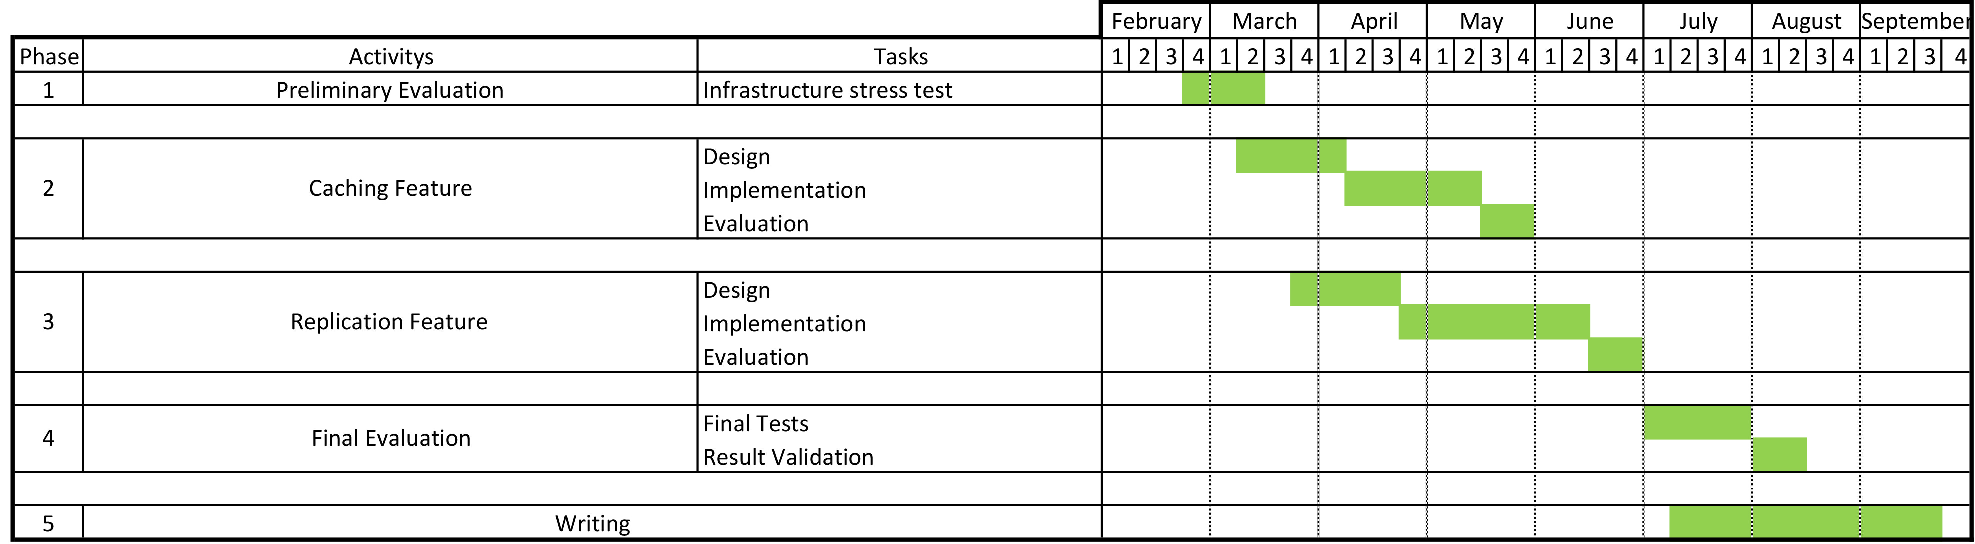
\includegraphics[width=\linewidth]{cap3_crono}
%	\caption{Proposed schedule of activities}
%	\label{fig:crono}
%\end{figure}	
%\end{landscape}




% section work_plan (end)
